\chapter{近似逻辑综合研究}

\section{将近似乘法器直接应用于大型设计存在的问题}

即使设计的近似乘法器在经过评估后硬件开销较低,但基于该乘法器设计的DNN加速器可能硬件成本并不领先。例如,在图\ref{AC:AM:Adapt:Fig:LeNet_PDA_accuracy}中,PPAM(1,1)的PDA比XFYW和XWYF都要高,但在如图\ref{AC:AM:Adapt:Fig:Acc_TASU}所示的基于不同乘法器的TASU加速器的\cite{Accelerator:JiaoLi}硬件开销比较中,基于PPAM(1,1)的设计比基于乘法器\emph{`A'}、\emph{`B'}、\emph{`C'}的PDA都要低,这是因为当近似乘法器作为一个模块放在电路中时,EDA工具能够根据不同的电路执行不同的优化,因此有必要对基于不同近似乘法器的DNN加速器的硬件成本进行探究。

\section{基于近似乘法器库面向 DNN 加速器的近似逻
辑综合}

将提出的基于MFFC自适应超图划分的端到端强化学习逻辑优化框架与近似乘法器库结合,针对DNN硬件加速器,本文首先对图\ref{AC:AM:Adapt:Fig:LeNet_PDA_accuracy}中共68个XWYF近似乘法器利用DC在7nm工艺库\cite{ASAP7_github}上基于2GHz的时钟频率约束进行综合以获取PDA,找到位于帕累拖前沿的乘法器;之后对基于不同乘法器的68个卷积操作加速单元SC\cite{Accelerator:SC}利用提出的开源逻辑优化框架进行优化,获取ADP并比较结果。


\section{实验结果}

\begin{figure}[!htb]
    \centering
    \subfigure[XWYF乘法器的评估结果]{
    \label{AC:ALS:Fig:LeNet_XWYF}
    \begin{minipage}[t]{0.48\linewidth}
    \centering
    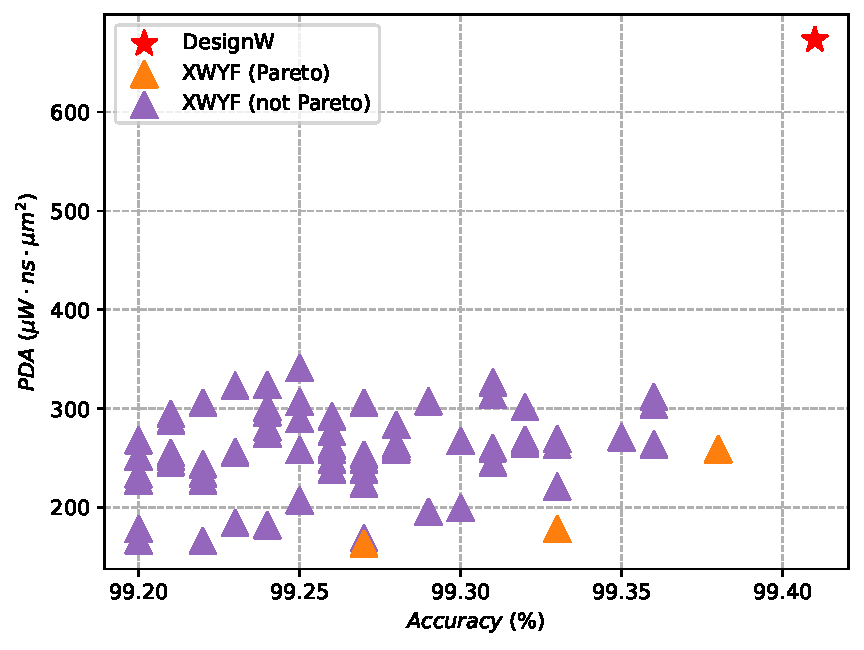
\includegraphics[width=\linewidth]{figs/LeNet_XWYF_PDA.pdf}
    \end{minipage}
    }
    \subfigure[基于XWYF实现的卷积加速器的评估结果]{
    \label{AC:ALS:Fig:SC}
    \begin{minipage}[t]{0.48\linewidth}
    \centering
    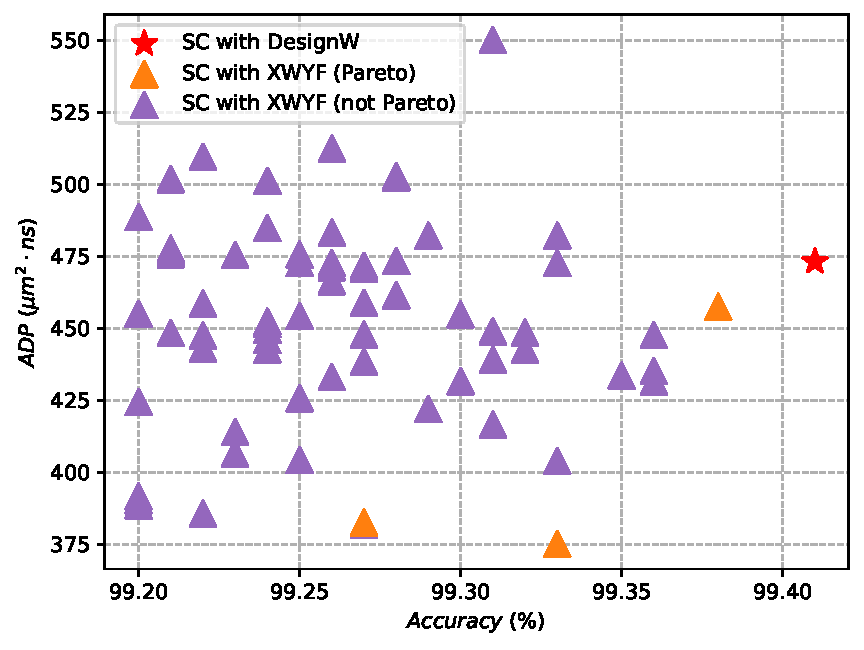
\includegraphics[width=\linewidth]{figs/SC_LeNet_XWYF_ADP.pdf}
    \end{minipage}
    }
\caption{XWYF乘法器的评估结果以及基于XWYF实现的卷积加速器的评估结果}
\label{AC:ALS:Fig:SC_LeNet_XWYF}
\end{figure}

图\ref{AC:ALS:Fig:SC_LeNet_XWYF}展示了68个XWYF乘法器的评估结果以及基于XWYF实现的68个卷积加速器SC\cite{Accelerator:SC}的评估结果,作为对比,基于DesignWare库\cite{IP:DesignWare}实现的精确乘法器DesignW也被纳入比较。图\ref{AC:ALS:Fig:LeNet_XWYF}中共有3个乘法器位于帕累拖前沿,以黄色三角形表示,对应的SC实现在图\ref{AC:ALS:Fig:SC}中也以黄色三角形表示。一个有意思的现象是,虽然DesignW的单独评估结果显示其PDA较高,但基于DesignW实现的SC模块的硬件开销却优于相当一部分的XWYF乘法器,这说明了近似乘法器库在使用时不能简单地根据单独的硬件成本直接选择,而是应该进行多次尝试后决定。
图\ref{AC:ALS:Fig:SC}表明,基于3个帕累拖最优的乘法器的SC实现仍然位于帕累拖前沿,因此当给定一个近似乘法器库进行综合时,可对库中位于帕累拖前沿的乘法器进行一定次数的随机搜索,综合比较后选择最好的那个进行实现。


\section{本章小结}

本章将提出的逻辑优化框架与近似乘法器库结合,对基于不同近似乘法器的DNN硬件加速器进行研究,结果显示乘法器和加速器之间的性能收益存在不匹配的现象,即乘法器本身的硬件开销低,基于该乘法器实现的加速器的硬件开销不一定低,因此近似乘法器库在使用时不能简单地根据乘法器的单独硬件成本直接选择,而是应该进行多次尝试后决定。虽然本章的工作是基于ASIC近似乘法器进行的,但该方法可以很轻松的被迁移到基于FPGA近似乘法器的近似逻辑综合的研究上。